\begin{frame}
	\frametitle{Biosphäre - Lebewesen}

	\begin{figure}
		\centering
		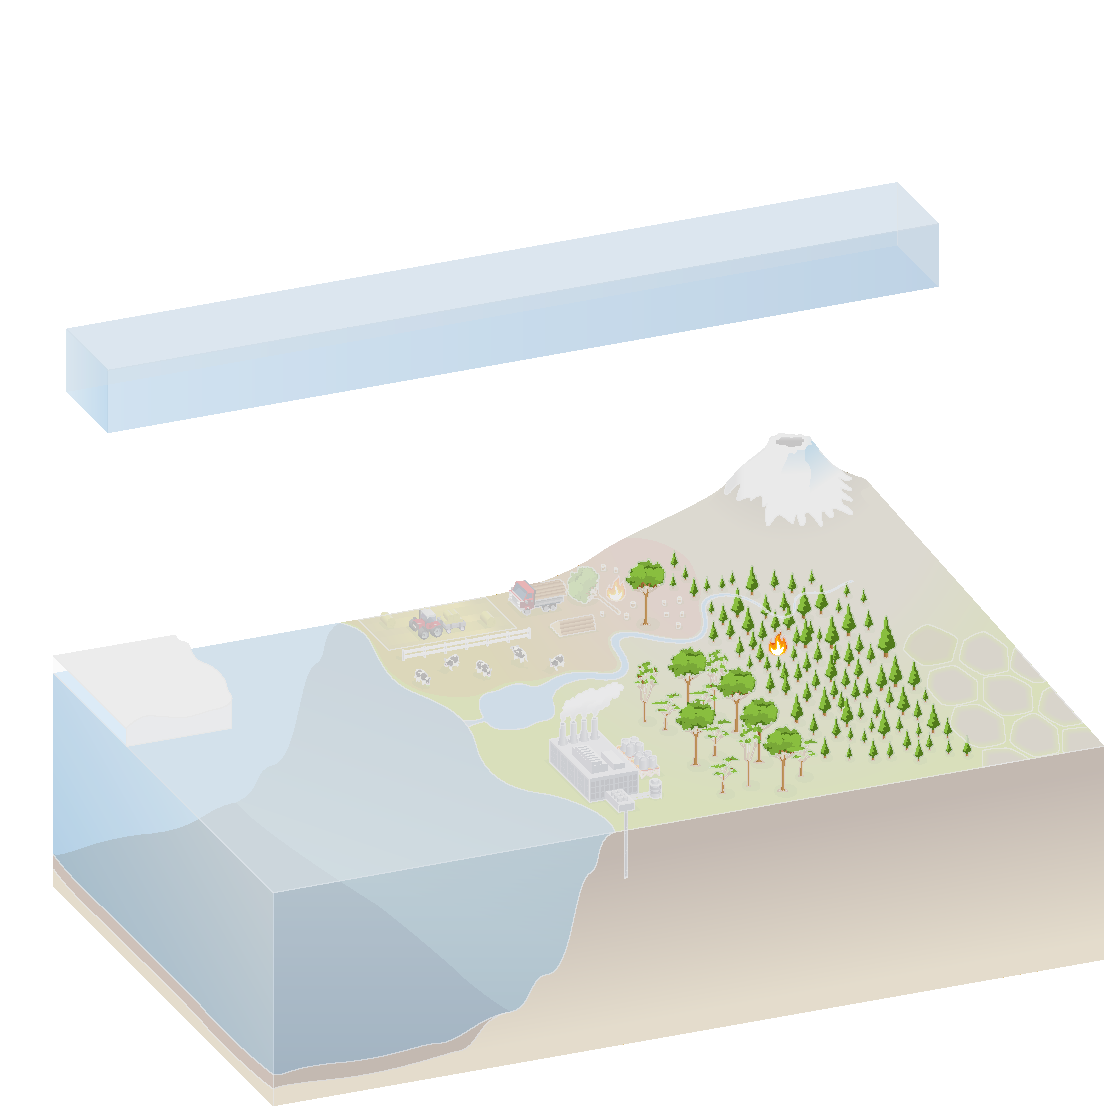
\includegraphics[trim={1cm 0cm 0cm 3cm}, clip, width=0.55\linewidth]{%
        bilder/climate_components/global_climate_components_biosphere.pdf}
		\caption{Die Vegetation ist eine interaktive Komponente des Klimasystems}
	\end{figure}

	\note{
		\begin{itemize}
			\item[] Umfasst sämtliches Leben auf der Erde
			\item[] Es zählen große Lebewesen, aber z.B. auch Mikroorganismen dazu
			\item[] Ersteckt sich vom Meeresboden bis in viele Kilometer Höhe
			\item[] Läßt sich vielfach untergliedern
			\item[] Vegetation ist sehr umfangreich und vielseitig
			\item[] bietet Lebensraum und Lebensgrundlage
			\item[] Auf der Erde die einzige uns bekannte Biosphäre
		\end{itemize}
	}
\end{frame}

\begin{frame}
	\frametitle{Biosphäre - Wechselwirkungen}
	\begin{columns}
		\column[t]{0.33\linewidth}
			\begin{itemize}
				\item Zahl der Tiere wirkt sich z.B. auf Methanausstoß aus
				\item Hängt selbst von Nahrungsangebot und menschlichem Einfluss ab
				\item Beweidung kann zu Albedoänderung führen
			\end{itemize}
			\begin{figure}
				\centering
				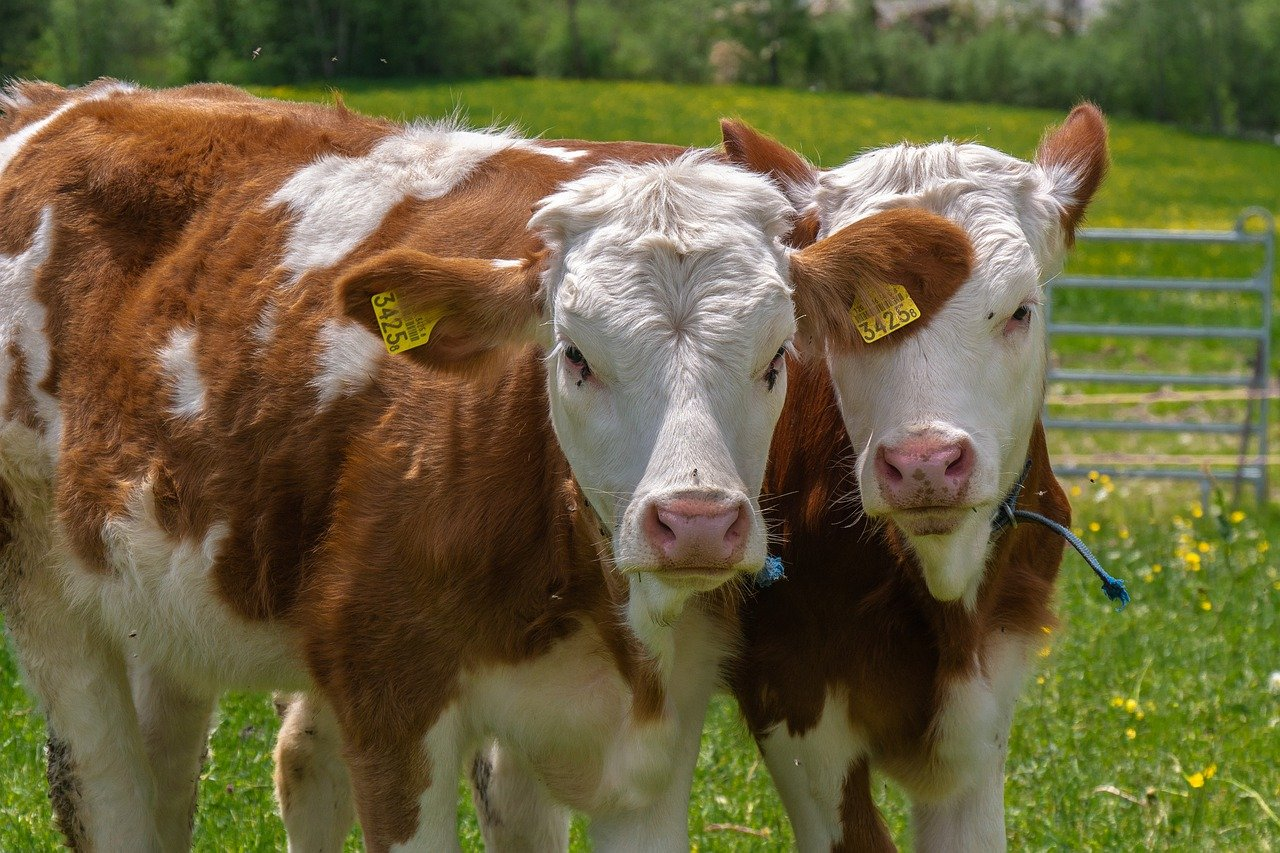
\includegraphics[width=\linewidth]{bilder/kuehe}
			\end{figure}
		\column[t]{0.33\linewidth}
			\begin{itemize}
				\item Ozeane können CO$_2$ aufnehmen
				\item Säuregehalt wirkt sich auf Leben im Wasser aus
				\item Auch Lebewesen selbst beeinflussen Bedingungen
			\end{itemize}
			\begin{figure}
				\centering
				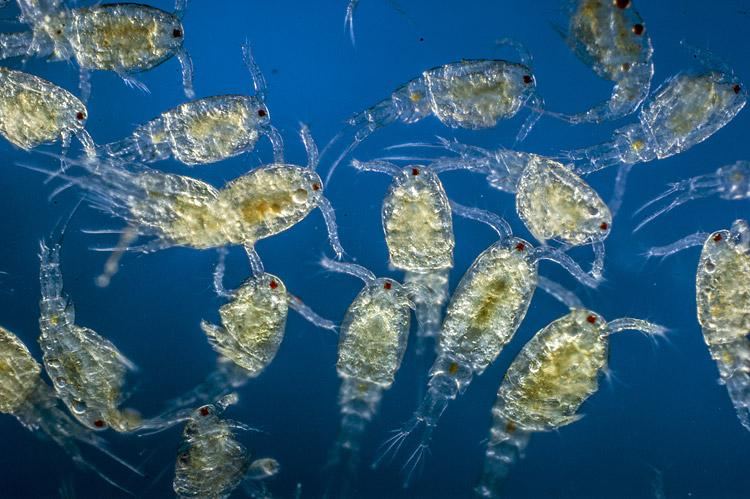
\includegraphics[width=\linewidth]{bilder/plankton}
			\end{figure}
		\column[t]{0.33\linewidth}
			\begin{itemize}
				\item Pflanzen sind Kohlenstoffsenken
				\item Bewuchs wirkt sich auf Albedo aus
				\item Wälder haben starken Einfluss aus lokales Klima
			\end{itemize}
			\begin{figure}
				\centering
				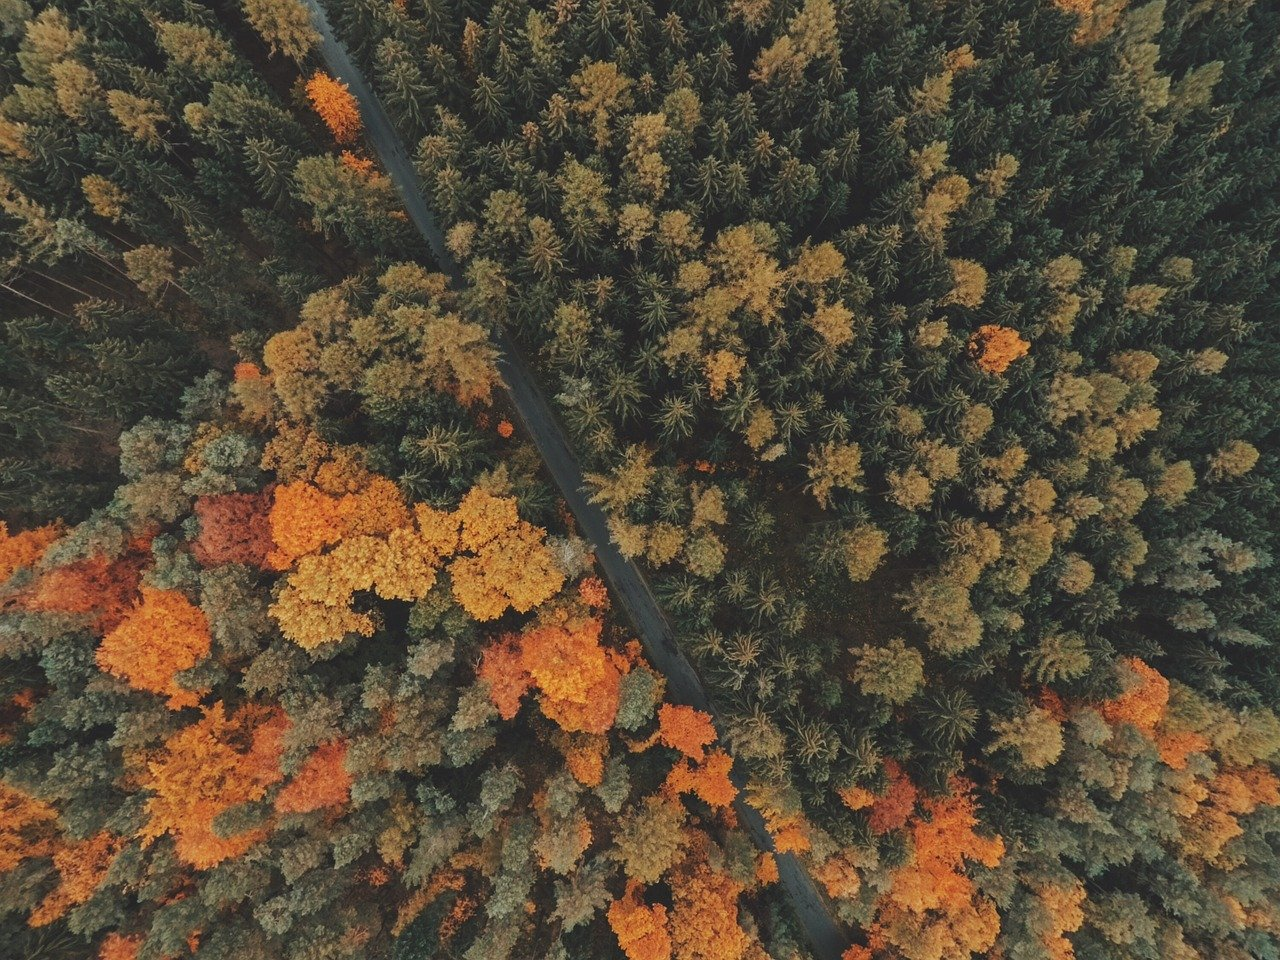
\includegraphics[width=\linewidth]{bilder/baeume}
			\end{figure}
	\end{columns}

	
	\note{
		\begin{itemize}
			\item[] steht in direktem Kontakt mit unterer Atmosphäre und Böden
			\item[] durch photosynthetische Prozesse und die Aufnahme sowie Abgabe von Wasser
			\item[] Vegetation hat dadurch massiven Einfluss auf Wetter und Klima - z.B. Tropischer Regenwald, Wolkenbildung
			\item[] zentral ist auch die Rolle beim Stoffkreislauf - u.a. Kohlenstoff, Phosphor, Nitrat, Stickstoff
		\end{itemize}
	}
\end{frame}
